
\documentclass[12pt, a4paper]{article}


%%%% Encodings

\usepackage[utf8]{inputenc} % encoding
\usepackage[english]{babel} % use special characters and also translates some elements within the document.

%%%% Misc

\usepackage{hyperref}       % Hyperlinks \url{url} or \href{url}{name}
\usepackage{parskip}        % \par starts on left (not idented)
\usepackage{tocbibind}      % Adds the bibliography to the table of contents (automatically)

% \usepackage[document]{ragged2e}  % Left-aligned (whole document)
% \begin{...} ... \end{...}   flushleft, flushright, center

%%%% Abstract

\usepackage{abstract}       % Abstract

% http://www.ctex.org/documents/packages/special/abstract.pdf
\renewcommand{\absnamepos}{flushleft} % \begin{abstract} \noindent ... \end{abstract}
\setlength{\absleftindent}{0pt}
\setlength{\absrightindent}{0pt}

%%%% Graphics

\usepackage{graphicx}
\graphicspath{ {./images/} } % directory to look up for graphics

% \begin{figure}[h]
%   \centering
%   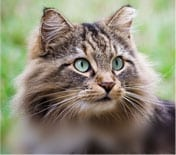
\includegraphics[scale=0.5]{cat}  % [width=\textwidth, height=4cm],
%   \caption{Example of a cat}
%   \label{fig:cat}
% \end{figure}

%%%% Math

\usepackage{amsmath}        % Math
\usepackage{amssymb}        % New symbols http://milde.users.sourceforge.net/LUCR/Math/mathpackages/amssymb-symbols.pdf
\usepackage{bm}             % $\bm{D + C}$

\usepackage{amsthm} % Math, \newtheorem, \proof, etc
% \begin{theorem}\label{t:label}  ...  \end{theorem}
% \begin{proof} ... \end{proof}
\theoremstyle{plain} % default
\newtheorem{theorem}{Theorem}[section]
\newtheorem{corollary}{Corollary}[theorem]  % Numering depends on the current section (instead of global)
\newtheorem{lemma}[theorem]{Lemma} % Shares numeration with theorem.
\theoremstyle{definition}
\newtheorem{definition}{Definition}[section]
\theoremstyle{remark}
\newtheorem*{remark}{Remark}

% Defines a new environment to write your or claim - proof
\newenvironment{claim}[1]{\par\noindent\underline{Claim:}\space#1}{}
\newenvironment{claimproof}[1]{\par\noindent\underline{Proof:}\space#1}{\hfill $\blacksquare$}

%%%% Code/Pseudo-code

\usepackage{minted} % Code listing
% \mint{html}|<h2>Something <b>here</b></h2>|
% \inputminted{octave}{BitXorMatrix.m}

%\begin{listing}[H]
  %\begin{minted}[xleftmargin=20pt,linenos,bgcolor=codegray]{haskell}
  %\end{minted}
  %\caption{Example of a listing.}
  %\label{lst:example} % You can reference it by \ref{lst:example}
%\end{listing}

\newcommand{\code}[1]{\texttt{#1}} % Define \code{foo.hs} environment

\usepackage[vlined,ruled]{algorithm2e} % pseudo-code http://tug.ctan.org/macros/latex/contrib/algorithm2e/doc/algorithm2e.pdf

%%%% Colors

\usepackage{xcolor}         % Colours \definecolor, \color{codegray}
\definecolor{codegray}{rgb}{0.9, 0.9, 0.9}
% \color{codegray} ... ...
% \textcolor{red}{easily}

%%%% Math

%\makeglossaries % before entries

%\newglossaryentry{latex}{
    %name=latex,
    %description={Is a mark up language specially suited
    %for scientific documents}
%}

% Referene to a glossary \gls{latex}
% Print glossaries \printglossaries

\usepackage[acronym]{glossaries} %

% \acrshort{name}
% \acrfull{name}
% \newacronym{foo}{arcshort}{acrfull}

\usepackage{enumitem}


\usepackage{fancyhdr}
\pagestyle{fancy}
\fancyhf{}
\rhead{Arnau Abella}
\lhead{AMMM}
\rfoot{Page \thepage}

\title{%
  \vspace{-12ex}
  \Large{Algorithmic Methods for Mathematical Models} \\
  \large{Lab Session 5 - GRASP Metaheuristics}
}
\author{%
  Arnau Abella \\
  \large{Universitat Polit\`ecnica de Catalunya}
}
\date{\today}

\begin{document}
\maketitle

\vspace{2ex}
\begin{enumerate}[label=(\alph*)]
    %%%%%%%%% a
    \item[\textcolor{QuestionBlue}{\textbullet}] \textcolor{QuestionBlue}{Prepare a pseudocode for the GRASP constructive algorithm. Specify the greedy function and the RCL.}

    \begin{algorithm}[H]
      \SetAlgoLined
      \DontPrintSemicolon
      \SetKwInput{Input}{Input}
      \SetKwInput{Output}{Output}
      \Input{
        \begin{itemize}
            \item A set $T$ of tasks, each task $t$ requires $r_{t}$ resources
            \item A set $C$ of computers, each computer $c$ has a capacity of $r_{c}$ resources
            \item The RCL threshold parameter $\alpha \in [0, 1]$
        \end{itemize}
      }
      \Output{
        A set $w$ of assignments, each assignment $\angles{t, c}$ associates a task $t$ with a computer $c$ \textit{s.t.} Each task $t \in T$ appears exactly once
      }
      $w \leftarrow \emptyset$\;
      \ForAll{$t \in T$}{
        $Q \leftarrow \{ \angles{c, q(\angles{t, c}, w)}  \ | \ c \in C, q(\angles{t, c}, w) \neq \infty \}$\;
        \If{$|Q| = 0$}{
          \Return{$INFEASIBLE$}\;
        }\;
        $q^{min} \leftarrow \min_{q} Q$\;
        $q^{max} \leftarrow \max_{q} Q$\;
        $RCL \leftarrow \{ c \in Q \ | \  q(\angles{t, c}, w) \leq q^{min} + \alpha(q^{max} - q^{min}) \}$\;
        $c_{sel} \leftarrow$  \textit{u.a.r} select $c \in RCL$\;
        $w \leftarrow w \cup \{ \angles{t, c_{sel}}\}$\;
      }

      \Return{$w$}\;
      \caption{GRASP - Constructive Algorithm}
    \end{algorithm}

    \begin{figure}[H]
      \begin{align*}
        &q(\angles{t, c}, w) =
          \begin{cases}
            \infty& if r_{t} > r_{c} - \sum_{t' \in w_{c}}r_{t'}  \\
            \frac{r_{t} + \sum_{t' \in w_{c}}r_{t'}}{r_{c}} & otherwise
          \end{cases}
      \end{align*}
      % \caption{Cost function}
    \end{figure}

    where $w_{c} = \{t_{i}, \ldots, t_{j} \} \subseteq T$ are the tasks assigned to computer $c$ in the partial solution $w$.

    %%%%%%%%% b
    \item[\textcolor{QuestionBlue}{\textbullet}] \textcolor{QuestionBlue}{Tune parameter $\alpha$. Generate at least 2 new random instances of medium size and run the constructive phase of GRASP for different  values of a from 0-1 in steps of 0.1. For every value, run the algorithm at least three times and compute the average of the cost of the obtained solutions. Prepare plots with the obtained values. Find the best value of $\alpha$ and use it for the rest of experiments.}

    The solution's quality in terms of $\alpha \in [0,1]$ has a v-shape with best value at $\alpha = 0.5$.

    \begin{figure}[H]
      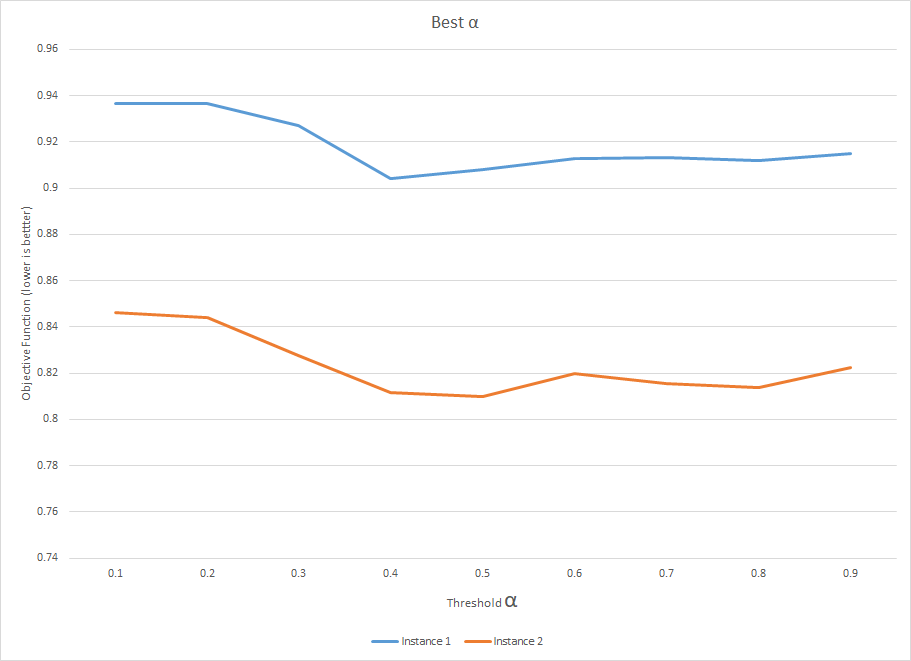
\includegraphics[width=\textwidth]{b}
      \caption{Objective value in terms of threshold $\alpha$}
      \label{fig:b}
    \end{figure}

    %%%%%%%%% c
    \item[\textcolor{QuestionBlue}{\textbullet}] \textcolor{QuestionBlue}{Solve the same instances that you generated in the last lab session using:
      \begin{itemize}
          \item Constructive phase only.
          \item Constructive + Local search (do for all combinations)
      \end{itemize}
    Configure the heuristics to stop after 10min and plot the quality of the solutions, the number of iterations performed, and the time to solve against the size of the instances.}

    The quality of the solution, in average, is better in the \textit{Constructive + LS} algorithm (see figure \ref{fig:c}).
    It is important to notice that although you are doing less iterations \i.e. narrower searches, the searches are more exhaustive
    in the neighbor of the solution (see table \ref{tab:c}).

    \begin{figure}[H]
      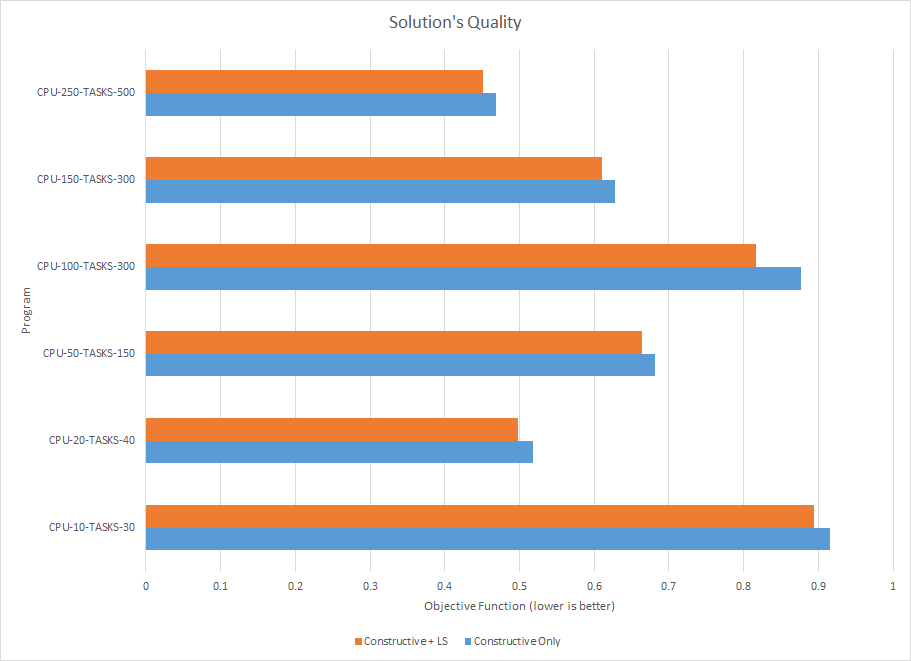
\includegraphics[width=\textwidth]{c}
      \caption{Constructive vs. Constructive + LS}
      \label{fig:c}
    \end{figure}

    \begin{table}[H]
    \centering
    \begin{tabular}{|c|c|c|}
      \hline
      Program           & \multicolumn{2}{c|}{Iterations}  \\ \hline
                        & Constructive & Constructive + LS \\ \hline
      CPU-10-TASKS-30   & 21313        & 4335              \\ \hline
      CPU-20-TASKS-40   & 4024         & 370               \\ \hline
      CPU-50-TASKS-150  & 227          & 10                \\ \hline
      CPU-100-TASKS-300 & 28           & 3                 \\ \hline
      CPU-150-TASKS-300 & 47           & 2                 \\ \hline
      CPU-250-TASKS-500 & 3            & 2                 \\ \hline
    \end{tabular}
    \caption{Iterations: Constructive vs. Constructive + LS}
    \label{tab:c}
    \end{table}

    %%%%%%%%% d
    \newpage
    \item[\textcolor{QuestionBlue}{\textbullet}] \textcolor{QuestionBlue}{Compare the results with those obtained in the previous lab session using greedy + LS and CPLEX.}

    In this particular problem, \textit{CPLEX} always performs better, in terms of execution time and solutions' quality, than the \textit{heuristic algorithms}. Among the heuristic algorithms, \textit{GRASP} performs better in term of solutions' quality than the \textit{greedy algorithm}.

    \begin{figure}[H]
      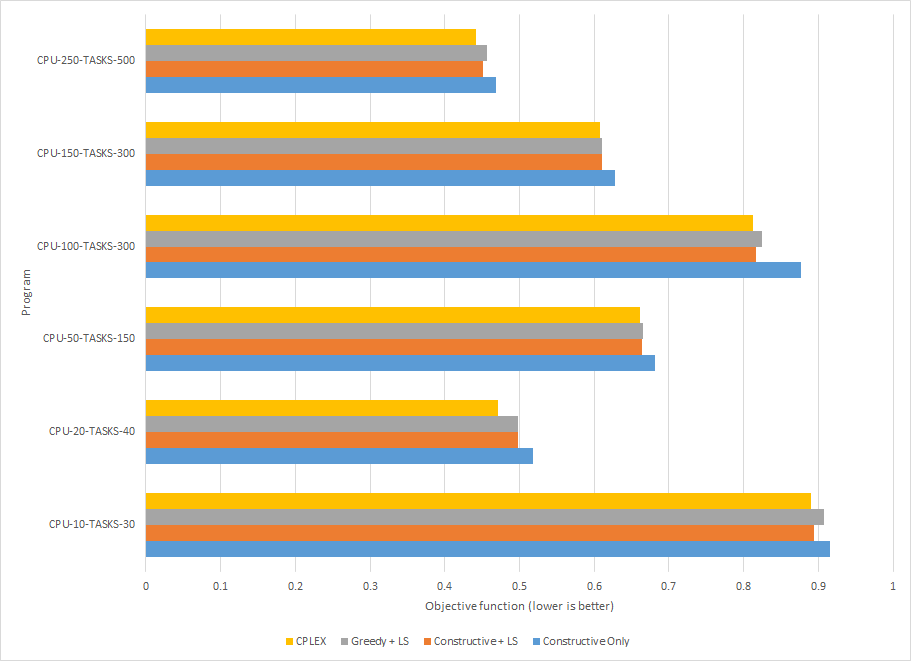
\includegraphics[width=\textwidth]{d}
      \caption{Comparison between Constructive, \mbox{Constructive + LS}, \mbox{Greedy + LS} and \mbox{ILP (CPLEX)}}
      \label{fig:d}
    \end{figure}

\end{enumerate}
\end{document}
